%******************************************************************************%
%                                                                              %
%                  html_css.en.tex for LaTeX                             %
%                  Created on : Tue Mar 10 13:27:28 2015                       %
%                  Made by : Dax Wann                                          %
%                                                                              %
%******************************************************************************%

\documentclass{42-en}

%******************************************************************************%
%                                                                              %
%                                    Header                                    %
%                                                                              %
%******************************************************************************%
\begin{document}



                           \title{Web Design with Basic HTML and CSS}
                          \subtitle{How to create and deploy a basic static website}
                       \member{Dax Wann}{daxwann@gmail.com}
                        \member{42 Staff}{pedago@42.fr}

\summary {
  An introduction to designing responsive websites with HTML and CSS.
}

\maketitle

\tableofcontents


%******************************************************************************%
%                                                                              %
%                                  Foreword                                    %
%                                                                              %
%******************************************************************************%
\chapter{Foreword}

    \begin{figure}[H]
        \begin{center}
            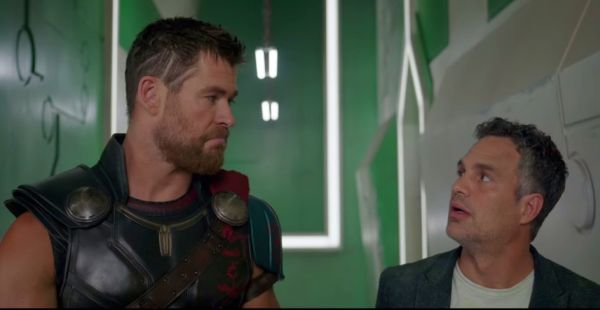
\includegraphics[width=12cm]{thor.jpg}
        \end{center}
    \end{figure}
    [Thor is trying to access on the Quinjet’s computer]\\
Quinjet Computer: Welcome. Voice activation required.\\
Thor: Thor.\\
Quinjet Computer: Access denied.\\
Thor: Thor, son of Odin.\\
Quinjet Computer: Access denied.\\
Thor: God of Thunder.\\
Quinjet Computer: Access denied.\\
Thor: Strongest Avenger.\\
Quinjet Computer: Access denied.\\
Thor: Strongest Avenger.\\
Quinjet Computer: Access denied.\\
Thor: Damn you, Stark. Point Break.\\
Quinjet Computer: Welcome, Point Break.\\
\\
- \textit{Thor: Ragnarok}
    
%******************************************************************************%
%                                                                              %
%                                 Introduction                                 %
%                                                                              %
%******************************************************************************%
\chapter{Introduction}

It's time to learn how to build a website for the world to see! We will first focus on making a static website. A simple static website consists of HTML (HyperText Markup Language) and CSS (Cascading Style Sheet). HTML is used to create the structure of the website, such as text, images, and other media. CSS is used to style those structures, such as changing the color of the text, the size of the images, and layout of the page.\\
    
\textbf{HTML}: structure and content of the website\par
\textbf{CSS}: style and layout of the website\\

With the skills of using HTML and CSS, you will be able to design websites that's appealing, accessible, and responsive to the user's devices.



%******************************************************************************%
%                                                                              %
%                                  Goals                                       %
%                                                                              %
%******************************************************************************%
\chapter{Goals}

Using FreeCodeCamp online curriculum, we will learn:
\begin{itemize}
    \item basic HTML
    \item basic CSS
    \item applied visual design
\end{itemize}

For our culminating project, we will apply what we learned to design and create a static web page about how to cook a dish of your choice. We will push our project onto a Github repository and deploy our website with Github Pages to showcase.



%******************************************************************************%
%                                                                              %
%                             General instructions                             %
%                                                                              %
%******************************************************************************%
\chapter{General instructions}

\begin{itemize}
    \item Make sure you can explain to your peers about how you built your recipe page using HTML and CSS
    \item Reflect on what you learned in FreeCodeCamp and how you applied it to your project
\end{itemize}
   
    



%******************************************************************************%
%                                                                              %
%                             Mandatory part                                   %
%                                                                              %
%******************************************************************************%
\chapter{Mandatory part}

Finish all exercises in these following sections on FreeCodeCamp Responsive Web Design Certificate:
\begin{itemize}
    \item Basic HTML and HTML5
    \item Basic CSS
    \item Applied Visual Design
\end{itemize}
\vspace{0.2in}

Create a static web page about instructions to cook a dish of your choice.\par
\vspace{0.2in}
Push your website project repository onto your Github. Deploy your website on github.io.
    


%******************************************************************************%
%                                                                              %
%                             Exercises of a Piscine                           %
%                                                                              %
%******************************************************************************%

\chapter{Exercise 00: FreeCodeCamp}

\extitle{Sign up on \href{FreeCodeCamp}{FreeCodeCamp}}
\exnumber{\exercicenumber}
\exscore{2}
\exfiles{n/a}
\exauthorize{All}

\makeheaderfiles

Go to \url{https://www.freecodecamp.org/} and create an account using a personal email. In "Curriculum", go to Responsive Web Design Certificate section.

%******************************************************************************%
%                                                                              %
%                             Exercises of a Piscine                           %
%                                                                              %
%******************************************************************************%

\chapter{Exercise 01: Basic HTML and HTML5}

\extitle{Basic HTML and HTML5 on FreeCodeCamp}
\exnumber{\exercicenumber}
\exscore{2}
\exfiles{All exercises completed in section on FreeCodeCamp}
\exauthorize{All}

\makeheaderfiles

HTML is used to create a structure for contents in the website. Usually websites will have a header and a body. A website can also include text, images, videos, and other media.

%******************************************************************************%
%                                                                              %
%                             Exercises of a Piscine                           %
%                                                                              %
%******************************************************************************%

\chapter{Exercise 02: Basic CSS}

\extitle{Basic CSS on FreeCodeCamp}
\exnumber{\exercicenumber}
\exscore{2}
\exfiles{All exercises completed in section on FreeCodeCamp}
\exauthorize{All}

\makeheaderfiles

CSS is used to style the structures created in HTML. For example, we use CSS to change fonts, text sizes, background color, image sizes, etc. We also use CSS to create overall layout of the website. You will learn more layout functionalities later with CSS Flexbox and CSS Grid.

%******************************************************************************%
%                                                                              %
%                             Exercises of a Piscine                           %
%                                                                              %
%******************************************************************************%

\chapter{Exercise 03: Applied Visual Design}

\extitle{Applied Visual Design on FreeCodeCamp}
\exnumber{\exercicenumber}
\exscore{2}
\exfiles{All exercises completed in section on FreeCodeCamp}
\exauthorize{All}

\makeheaderfiles

We will now learn more about designing a website using CSS. A website would be frustrating for the users if its design was not well thought out. For example, we should make the text big enough for users to read easily. We should highlight the important content. We should use colors and images to support our main content.

%******************************************************************************%
%                                                                              %
%                             Exercises of a Piscine                           %
%                                                                              %
%******************************************************************************%

\chapter{Exercise 04: Food Recipe Page}

\extitle{Teach someone to cook a dish with a web page}
\exnumber{\exercicenumber}
\exscore{2}
\exfiles{Your project folder should include index.html, style.css, and image files in "assets/" subdirectory}
\exauthorize{All}

\makeheaderfiles

Create an instructions page on how to cook a dish of your choice. You can get recipe, images, and instructions from an existing cooking website.\par
\vspace{.1in}
The website should have:
\begin{itemize}
    \item a heading
    \item one or more images of the dish
    \item an unordered (bullet) list of ingredients
    \item an ordered (numbered) list of instructions
    \item a link to the website where you got the information from
    \item a footer that includes your name
\end{itemize}
\vspace{.5in}
Use the wireframes below for inspiration
\begin{figure}[H]
    \begin{center}
        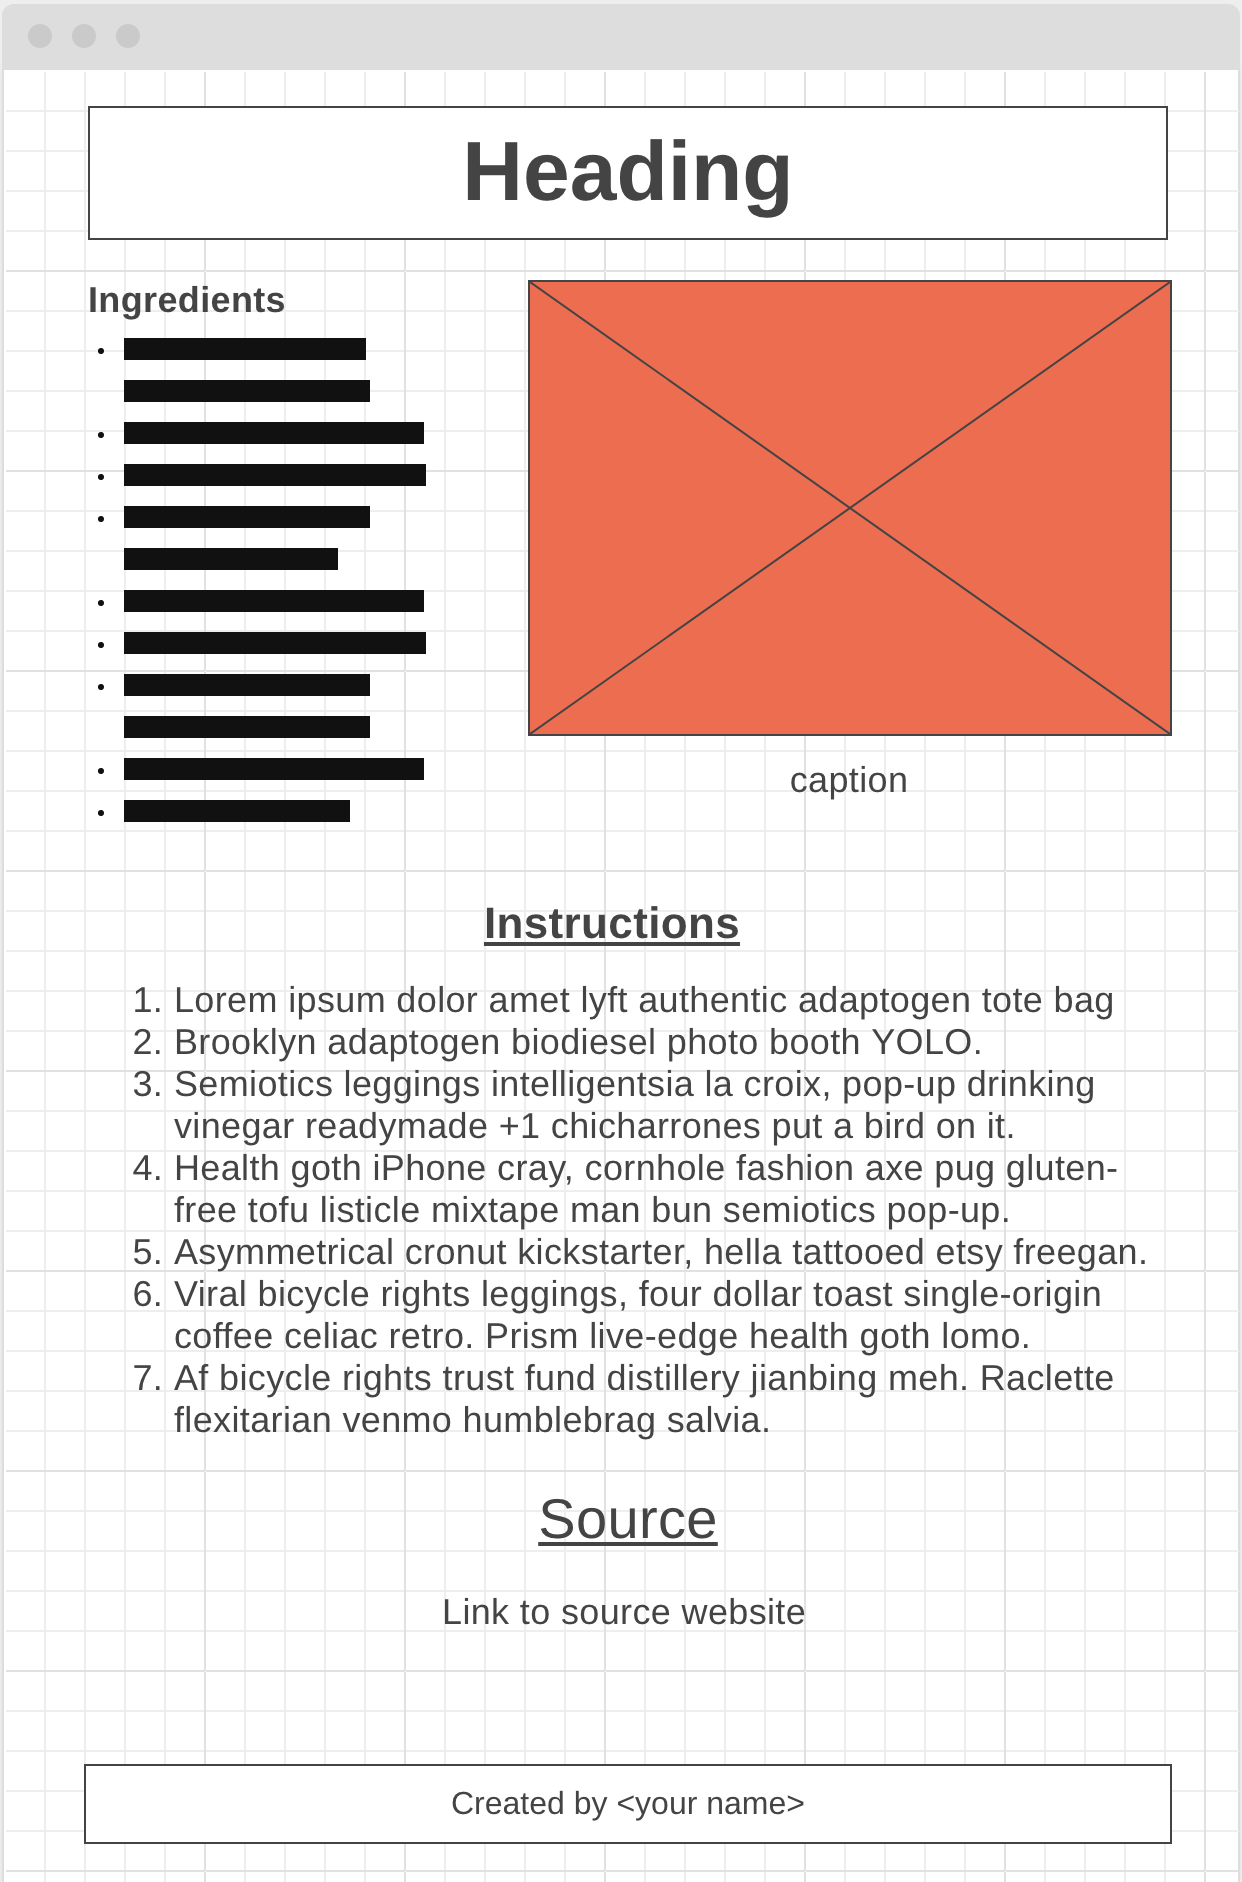
\includegraphics[width=14cm]{wireframe.png}\\
        desktop view
    \end{center}
\end{figure}
\textbf{Suggestions}
\begin{enumerate}
    \item Create a project folder along with files \texttt{index.html} and \texttt{style.css}. Create a subfolder named \texttt{assets/} for images
    \item Use Visual Studio Code IDE to open the folder and start writing the HTML and CSS
    \item Apply what you learned in FreeCodeCamp to create the structure of the website and style it
    \item Use Chrome browser to test your website. You can access your website by opening the html file with Chrome or typing in its file path in the browser. If you are stuck, google first.
\end{enumerate}

%******************************************************************************%
%                                                                              %
%                             Exercises of a Piscine                           %
%                                                                              %
%******************************************************************************%

\chapter{Exercise 05: Github}

\extitle{Create github account}
\exnumber{\exercicenumber}
\exscore{2}
\exfiles{Your Github repository should include \texttt{index.html}, \texttt{style.css}, and image files in \texttt{assets/} subdirectory}
\exauthorize{All}

\makeheaderfiles

\begin{enumerate}
    \item Go to \url{https://github.com/} and create a free account using your personal email if you don't already have one
    \item Create a new public repository named \texttt{H2S\_recipe\_page}
    \item Follow \href{https://help.github.com/en/articles/adding-a-remote}{instructions} on connecting your tribute website project to the new Github repository
    \item Push your project onto the Github repository
    \item Go to your Github repository settings, under "Github Pages", publish your project as a website. Follow the URL formatted as
    \begin{center}
        \texttt{<username>.github.io/H2S\_recipe\_page} \\
    \end{center}
    to view website.
    \item Create a \texttt{README.md} in the root directory of your project folder and copy the website URL into it. Follow this \href{https://help.github.com/en/articles/basic-writing-and-formatting-syntax#headings}{guide}.
\end{enumerate}

%******************************************************************************%
%                                                                              %
%                           Turn-in and peer-evaluation                        %
%                                                                              %
%******************************************************************************%
\chapter{Turn-in and peer-evaluation}

    Check that all exercises in the previously listed FreeCodeCamp sections have been completed.\\
    
    Check website is published on Github Pages.\\

    Turn your source code in using your \texttt{42 Git repository}. Only work present on your repository will be graded in defense.

%******************************************************************************%
\end{document}
